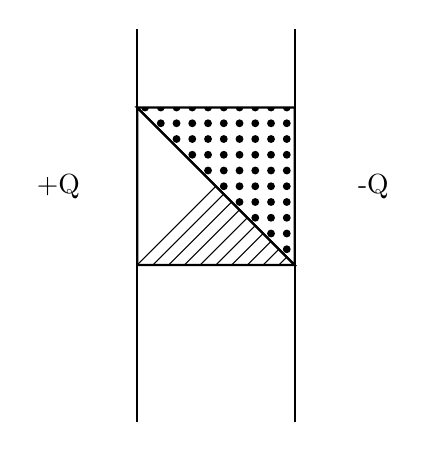
\begin{tikzpicture}
    % Draw the two parallel lines
    \draw[thick] (0,0) -- (0,5);
    \draw[thick] (2,0) -- (2,5);

    % Shaded area
   \begin{scope}
    % Clip to the first triangle
    \clip (0,2) -- (0,4) -- (2,2) -- cycle;
    % Draw diagonal lines
    \foreach \x in {-1, -0.8, ..., 3} { % Adjust range and spacing as needed
        \draw[thin] (\x,1) -- (\x+3,4); % Adjust angle and coverage
    }
\end{scope}
% Outline the first triangle
\draw[thick] (0,2) -- (0,4) -- (2,2) -- cycle;

% Second triangle with manual dots
\begin{scope}
    % Clip to the second triangle
    \clip (0,4) -- (2,2) -- (2,4) -- cycle;
    % Add dots manually using a foreach loop
    \foreach \x in {0.1,0.3,...,2.5} { % Adjust step size for spacing
        \foreach \y in {2.2,2.4,...,4.1} { % Adjust step size for density
            \fill (\x,\y) circle (0.05); % Adjust dot size
        }
    }
\end{scope}
% Outline the second triangle
\draw[thick] (0,4) -- (2,2) -- (2,4) -- cycle;
    % Labels
    \node at (-1,3) {+Q};
    \node at (3,3) {-Q};
\end{tikzpicture}
